\documentclass[12pt, a4paper]{article} 
\usepackage{tcolorbox}
\tcbuselibrary{skins, breakable, theorems}
\usepackage{subcaption}
\usepackage{pdflscape} 

\newtcbtheorem{question}{题~(理}%
  {enhanced, breakable,
    colback = white, colframe = cyan, colbacktitle = cyan,
    attach boxed title to top left = {yshift = -2mm, xshift = 5mm},
    boxed title style = {sharp corners},
    fonttitle = \sffamily\bfseries, separator sign = {).~}}{qst}
%\documentclass[12pt, a4paper]{article} 

\usepackage{fontspec} % Font selection for XeLaTeX; see fontspec.pdf. 
\usepackage{xeCJK}	% 中文使用 XeCJK,利用 \setCJKmainfont 定義中文內文、粗體與斜體的字型
\defaultfontfeatures{Mapping=tex-text} % to support TeX conventions like ``---''
\usepackage{xunicode} % Unicode support for LaTeX character names(accents, European chars, etc)
\usepackage{xltxtra} 				% Extra customizations for XeLaTeX
\usepackage{amsmath, amssymb}
\usepackage{enumerate}
\usepackage{graphicx,subfig,float,wrapfig} % support the \includegraphics command and options
\usepackage[outercaption]{sidecap} %[options]=[outercaption], [innercaption], [leftcaption], [rightcaption]
\usepackage{array, booktabs}
\usepackage{color, xcolor}
\usepackage{longtable}
\usepackage{colortbl}                          				
\usepackage{listings}						% 直接將 latex 碼轉換成顯示文字
\usepackage[parfill]{parskip} 				% 新段落前加一空行,不使用縮排
\usepackage[left=1.5in,right=1in,top=1in,bottom=1in]{geometry} 
%%%左邊比較長,寫論文時裝訂用
\usepackage{url}
%%%%%%%%%%%%%%%%%
\usepackage{graphicx}
\usepackage{caption}

\usepackage{adjustbox}%%%%表格系列的包
\usepackage{multicol}
\usepackage{multirow}
\usepackage{diagbox} % 用於創建斜線標題的宏包

%-----------------------------------------------------------------
%數學定理
% Counter
\usepackage{amsthm}	
\theoremstyle{plain}
\newtheorem{de}{Definition}[section]		%definition獨立編號
\newtheorem{thm}{{\MB 定理}}[section]		%theorem 獨立編號,取中文名稱並給予不同字型
\newtheorem{lemma}[thm]{Lemma}			%lemma 與 theorem 共用編號
\newtheorem{ex}{{\E Example}}				%example 獨立編號,不編入小節數字,走流水號。也換個字型。
\newtheorem{cor}{Corollary}[section]		%not used here
\newtheorem{exercise}{EXERCISE}			%not used here
\newtheorem{re}{\emph{Result}}[section]	%not used here
\newtheorem{axiom}{AXIOM}				%not used here
\renewcommand{\proofname}{\bf{Proof}}		%not used here
\newcounter{quiz}						% start a simple and new counter
\setcounter{quiz}{1}						% start to count from 1
				% start to count from 1


%-----------------------------------------------------------------
%  中英文內文字型設定
\setCJKmainfont							% 設定中文內文字型
	[
%		BoldFont=Microsoft YaHei	    %定義粗體的字型(Win)
		BoldFont=蘋果儷中黑	    		%定義粗體的字型(Mac)
	]
%	{新細明體}						% 設定中文內文字型(Win)
	{宋體-繁}							% 設定中文內文字型(Mac)	
\setmainfont{Times New Roman}		% 設定英文內文字型
\setsansfont{Arial}					% 無襯字字型 used with {\sffamily ...}
%\setsansfont[Scale=MatchLowercase,Mapping=tex-text]{Gill Sans}
\setmonofont{Courier New}			% 等寬字型 used with {\ttfamily ...}
%\setmonofont[Scale=MatchLowercase]{Andale Mono}
% 其他字型(隨使用的電腦安裝的字型不同,用註解的方式調整(打開或關閉))
% 英文字型
%\newfontfamily{\E}{Calibri}				
\newfontfamily{\A}{Arial}
\newfontfamily{\C}[Scale=0.9]{Arial}
\newfontfamily{\R}{Times New Roman}
\newfontfamily{\TT}[Scale=0.8]{Times New Roman}
% 中文字型
%\newCJKfontfamily{\MB}{微軟正黑體}				% 等寬及無襯線字體 Win
\newCJKfontfamily{\MB}{黑體-繁}				% 等寬及無襯線字體 Mac
%\newCJKfontfamily{\SM}[Scale=0.8]{新細明體}	% 縮小版(Win)
\newCJKfontfamily{\SM}[Scale=0.8]{宋體-繁}	% 縮小版(Mac)
%\newCJKfontfamily{\K}{標楷體}                	% Windows下的標楷體
\newCJKfontfamily{\K}{楷體-繁}               	% Mac下的標楷體
%\newCJKfontfamily{\BB}{Microsoft YaHei}		% 粗體 Win
\newCJKfontfamily{\BB}{蘋果儷中黑}		% 粗體 Mac
% 以下為自行安裝的字型:CwTex 組合
%\newCJKfontfamily{\CF}{cwTeX Q Fangsong Medium}	% CwTex 仿宋體
%\newCJKfontfamily{\CB}{cwTeX Q Hei Bold}			% CwTex 粗黑體
%\newCJKfontfamily{\CK}{cwTeX Q Kai Medium}   	% CwTex 楷體
%\newCJKfontfamily{\CM}{cwTeX Q Ming Medium}		% CwTex 明體
%\newCJKfontfamily{\CR}{cwTeX Q Yuan Medium}		% CwTex 圓體
%-----------------------------------------------------------------------------------------------------------------------
\XeTeXlinebreaklocale "zh"             		%這兩行一定要加,中文才能自動換行
\XeTeXlinebreakskip = 0pt plus 1pt     		%這兩行一定要加,中文才能自動換行
%-----------------------------------------------------------------------------------------------------------------------
\newcommand{\cw}{\texttt{cw}\kern-.6pt\TeX}	% 這是 cwTex 的 logo 文字
\newcommand{\imgdir}{/Users/heng/Documents/master_eco_thesis/master_thesis_latex/graph/}% 設定圖檔的目錄位置

\renewcommand{\tablename}{表}	% 改變表格標號文字為中文的「表」(預設為 Table)
\renewcommand{\figurename}{圖}% 改變圖片標號文字為中文的「圖」(預設為 Figure)

% 設定顏色 see color Table: http://latexcolor.com
\definecolor{slight}{gray}{0.9}				
\definecolor{airforceblue}{rgb}{0.36, 0.54, 0.66} 
\definecolor{arylideyellow}{rgb}{0.91, 0.84, 0.42}
\definecolor{babyblue}{rgb}{0.54, 0.81, 0.94}
\definecolor{cadmiumred}{rgb}{0.89, 0.0, 0.13}
\definecolor{coolblack}{rgb}{0.0, 0.18, 0.39}
\definecolor{beaublue}{rgb}{0.74, 0.83, 0.9}
\definecolor{beige}{rgb}{0.96, 0.96, 0.86}
\definecolor{bisque}{rgb}{1.0, 0.89, 0.77}
\definecolor{gray(x11gray)}{rgb}{0.75, 0.75, 0.75}
\definecolor{limegreen}{rgb}{0.2, 0.8, 0.2}
\definecolor{splashedwhite}{rgb}{1.0, 0.99, 1.0}

%---------------------------------------------------------------------
% 映出程式碼 \begin{lstlisting} 的內部設定
\lstset
{	language=[LaTeX]TeX,
    breaklines=true,
    %basicstyle=\tt\scriptsize,
    basicstyle=\tt\normalsize,
    keywordstyle=\color{blue},
    identifierstyle=\color{black},
    commentstyle=\color{limegreen}\itshape,
    stringstyle=\rmfamily,
    showstringspaces=false,
    %backgroundcolor=\color{splashedwhite},
    backgroundcolor=\color{slight},
    frame=single,							%default frame=none 
    rulecolor=\color{gray(x11gray)},
    framerule=0.4pt,							%expand outward 
    framesep=3pt,							%expand outward
    xleftmargin=3.4pt,		%to make the frame fits in the text area. 
    xrightmargin=3.4pt,		%to make the frame fits in the text area. 
    tabsize=2				%default :8 only influence the lstlisting and lstinline.
}

% 映出程式碼 \begin{lstlisting} 的內部設定 for Python codes
%\lstset{language=Python}
%\lstset{frame=lines}
%\lstset{basicstyle=\SCP\normalsize}
%\lstset{keywordstyle=\color{blue}}
%\lstset{commentstyle=\color{airforceblue}\itshape}
%\lstset{backgroundcolor=\color{beige}}   % 使用自己維護的定義檔
%-----------------------------------------------------------------------------------------------------------------------
% 文章開始
\title{ Teps-b資料統計}
\author{{\SM 鄭仲恒}}
\date{{\TT \today}} 	 
\begin{document}
\maketitle
\fontsize{12}{22 pt}\selectfont
Teps-b統計資料與圖形分析,CP代表原先調查為國中生族群,SH為原先調查高中生族群。文章先由CP核心資料先介紹,再後續介紹SH。

%%%%%%%%%%%%%%%%%%%%%%%%%%%%


\section{CP-核心資料國中生}
調查的資料分佈年份為2009、2013、2014、2019年,其中2014年度為專員實際進行面訪受訪者,其餘3次調查譏為電話訪談資料。
\subsection{2009年度調查-電訪}
變數資料經行統整,其中針對部分變數進行合併,重新標籤。

\begin{table}[htbp]
  \centering
   \caption{2009CP-樣本性別}
  \begin{adjustbox}{width=0.5\textwidth}
    \begin{tabular}{lcccc}
      \toprule
      TEPS-B & 樣本性別 & Freq. & Percent & Cum. \\
      \midrule
      & 男 & 1,764 & 49.10 & 49.10 \\
      & 女 & 1,829 & 50.90 & 100.00 \\
      \midrule
      Total & & 3,593 & 100.00 & \\
      \bottomrule
    \end{tabular}
  \end{adjustbox}
\end{table}

\bigskip

\begin{table}[htbp]
  \centering
  \caption{性別與學校類別}
  \begin{adjustbox}{width=\textwidth}
    \begin{tabular}{lcccccccccc}
      \toprule
      TEPS-B & 樣本性 & 大學 & 私立大學 & 國立科技 & 私立科技 & 技職學院 & 學院 & 國外大學 & 遺漏 & 跳答 \\
      \midrule
      & 男 & 424 & 528 & 100 & 256 & 150 & 16 & 9 & 178 & 103 \\
      & 女 & 350 & 639 & 77 & 247 & 162 & 8 & 25 & 230 & 91 \\
      \midrule
      Total & & 774 & 1,167 & 177 & 503 & 312 & 24 & 34 & 408 & 194 \\
      \bottomrule
    \end{tabular}
  \end{adjustbox}
\end{table}


\begin{figure}[h]
    \centering    
        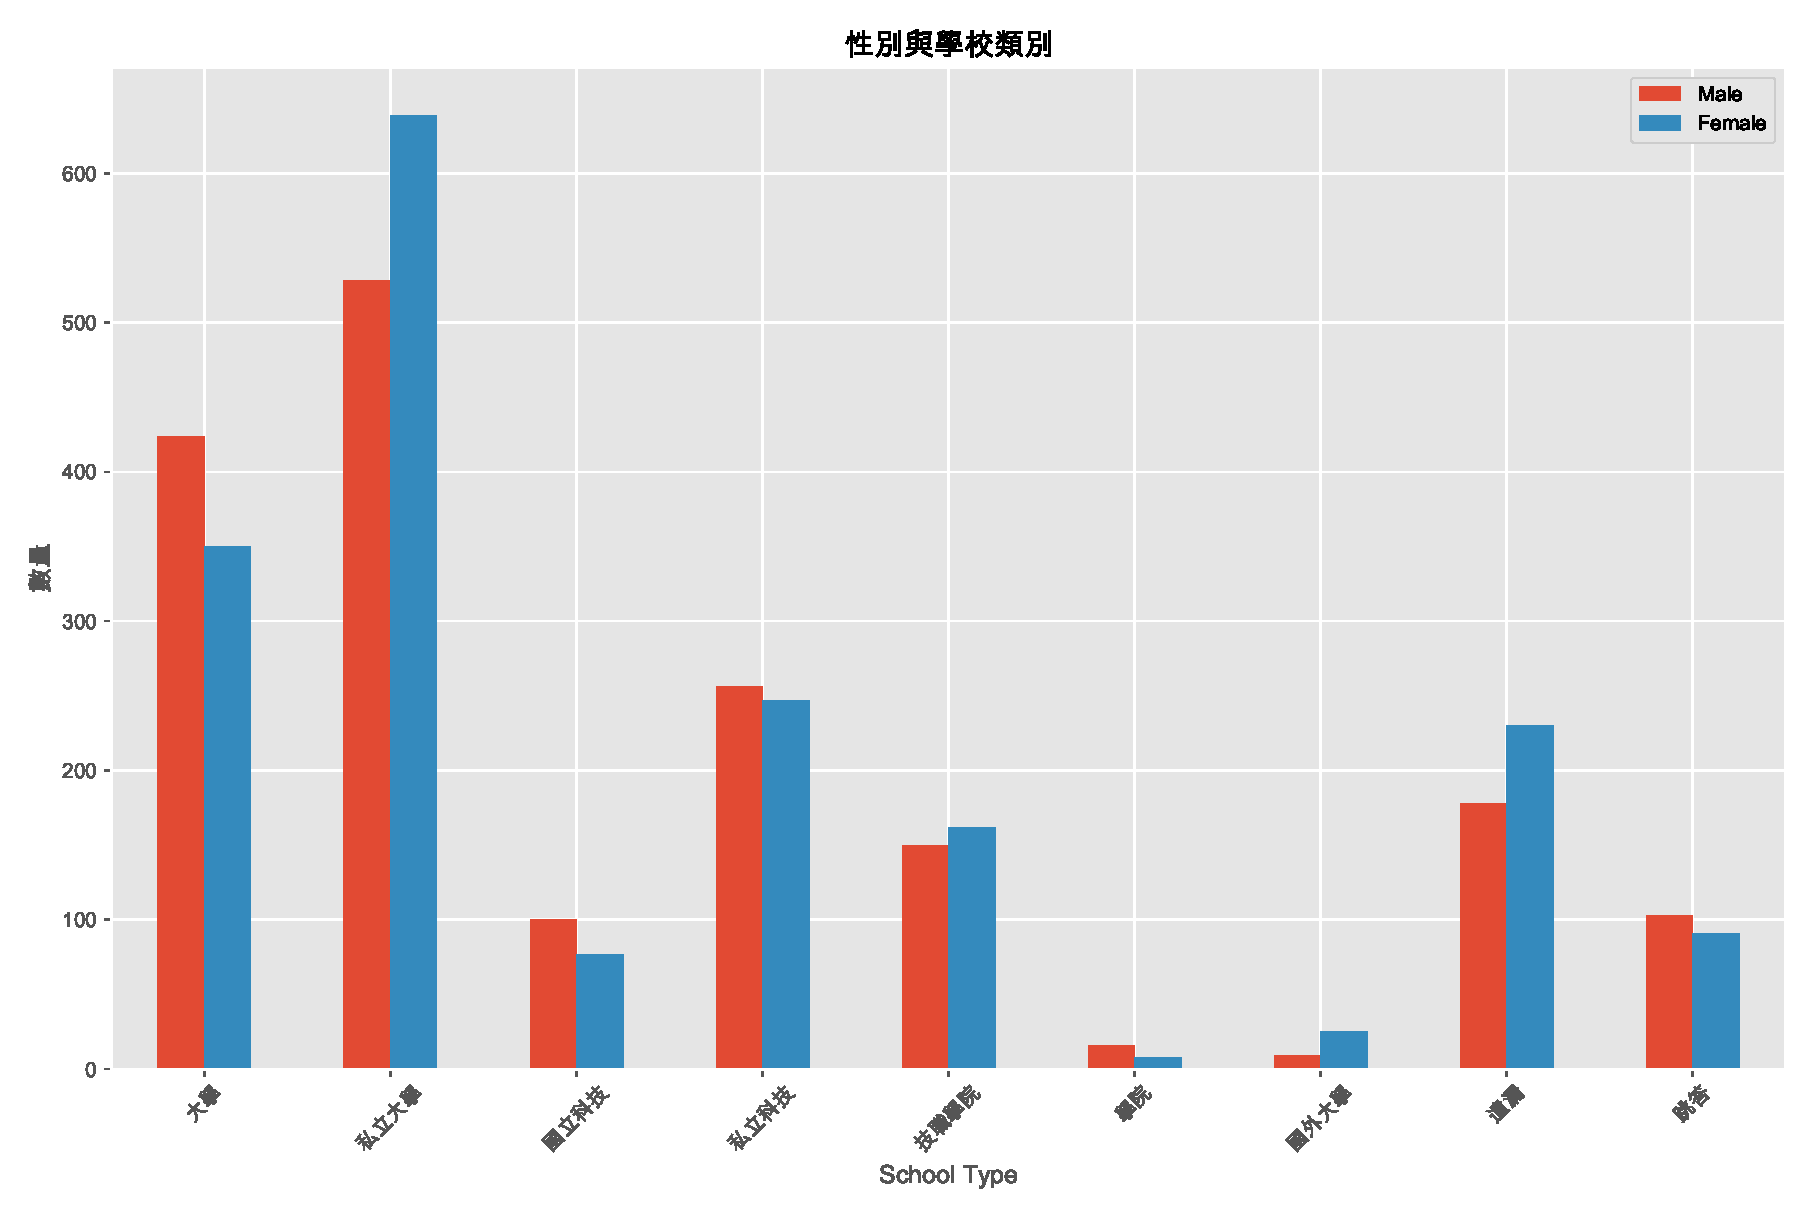
\includegraphics[width=\linewidth]{\imgdir/gender_school.eps}
        \caption{學校種類與薪酬}
        \label{pic:學校種類與薪酬}
\end{figure}









\begin{table}[ht]
\centering
\renewcommand{\arraystretch}{1.3} %%%把表格的高拉大
\extrarowheight=4pt
\caption{原始資料學歷與工作經驗}
\begin{adjustbox}{width=\textwidth}
\begin{tabular}{l*{8}{c}}
\toprule
& \multicolumn{8}{c}{受訪者工作(針對第一份工作計算)} \\
\cmidrule(lr){2-9}
\multirow{2}{*}{大學學校分類} & \multirow{2}{*}{遺漏、跳答、不清楚} & \multirow{2}{*}{5年} & \multirow{2}{*}{4年-5年} & \multirow{2}{*}{3年-4年} & \multirow{2}{*}{2年-3年} & \multirow{2}{*}{1年-2年} & \multirow{2}{*}{1年內} & \multirow{2}{*}{Total} \\
& &  &  &  &  & &  &  \\
\midrule
公立一般大學 & 773 & 0 & 0 & 1 & 0 & 0 & 0 & 774 \\
公立一般學院 & 18 & 0 & 0 & 0 & 0 & 0 & 0 & 18 \\
公立科技大學 & 176 & 0 & 0 & 0 & 0 & 1 & 0 & 177 \\
公立技職學院 & 70 & 0 & 0 & 0 & 2 & 2 & 0 & 74 \\
公立專科學校 & 20 & 0 & 0 & 0 & 0 & 0 & 0 & 20 \\
私立一般大學 & 1,152 & 1 & 1 & 0 & 5 & 8 & 0 & 1,167 \\
私立一般學院 & 6 & 0 & 0 & 0 & 0 & 0 & 0 & 6 \\
私立科技大學 & 480 & 1 & 1 & 1 & 15 & 3 & 2 & 503 \\
私立技職學院 & 198 & 0 & 0 & 2 & 7 & 3 & 0 & 210 \\
私立專科學校 & 8 & 0 & 0 & 0 & 0 & 0 & 0 & 8 \\
國外大學 & 31 & 0 & 0 & 0 & 0 & 0 & 0 & 31 \\
其他 & 3 & 0 & 0 & 0 & 0 & 0 & 0 & 3 \\
遺漏值 & 397 & 0 & 0 & 0 & 0 & 0 & 0 & 397 \\
不知道、不清楚 & 4 & 0 & 0 & 0 & 0 & 0 & 0 & 4 \\
拒答 & 7 & 0 & 0 & 0 & 0 & 0 & 0 & 7 \\
跳答 & 159 & 0 & 0 & 3 & 25 & 4 & 3 & 194 \\
Total & 3,502 & 2 & 2 & 7 & 54 & 21 & 5 & 3,593 \\
\bottomrule
\end{tabular}
\end{adjustbox}

\end{table}



\begin{table}[ht]
\centering
\renewcommand{\arraystretch}{1.3} %%%把表格的高拉大
\extrarowheight=4pt
\caption{學歷經分類與工作經驗}
\begin{adjustbox}{width=\textwidth}
\begin{tabular}{l*{8}{c}}
\toprule
& \multicolumn{8}{c}{受訪者工作(針對第一份工作計算)} \\
\cmidrule(lr){2-9}
\multirow{2}{*}{大學學校種類} & \multirow{2}{*}{遺漏、跳答、不清楚} & \multirow{2}{*}{5年} & \multirow{2}{*}{4年-5年} & \multirow{2}{*}{3年-4年} & \multirow{2}{*}{2年-3年} & \multirow{2}{*}{1年-2年} & \multirow{2}{*}{1年內} & \multirow{2}{*}{Total} \\
& &  &  &  &  &  &  &  \\
\midrule
國立大學 & 773 & 0 & 0 & 1 & 0 & 0 & 0 & 774 \\
私立大學 & 1,152 & 1 & 1 & 0 & 5 & 8 & 0 & 1,167 \\
國立科技大學 & 176 & 0 & 0 & 0 & 0 & 1 & 0 & 177 \\
私立科技大學 & 480 & 1 & 1 & 1 & 15 & 3 & 2 & 503 \\
技職學院、專科學校 & 296 & 0 & 0 & 2 & 9 & 5 & 0 & 312 \\
學院 & 24 & 0 & 0 & 0 & 0 & 0 & 0 & 24 \\
國外大學、其他 & 34 & 0 & 0 & 0 & 0 & 0 & 0 & 34 \\
遺漏、不清楚、拒答 & 408 & 0 & 0 & 0 & 0 & 0 & 0 & 408 \\
跳答 & 159 & 0 & 0 & 3 & 25 & 4 & 3 & 194 \\
Total & 3,502 & 2 & 2 & 7 & 54 & 21 & 5 & 3,593 \\
\bottomrule
\end{tabular}
\end{adjustbox}
\end{table}



\begin{figure}[H]
    \centering    
        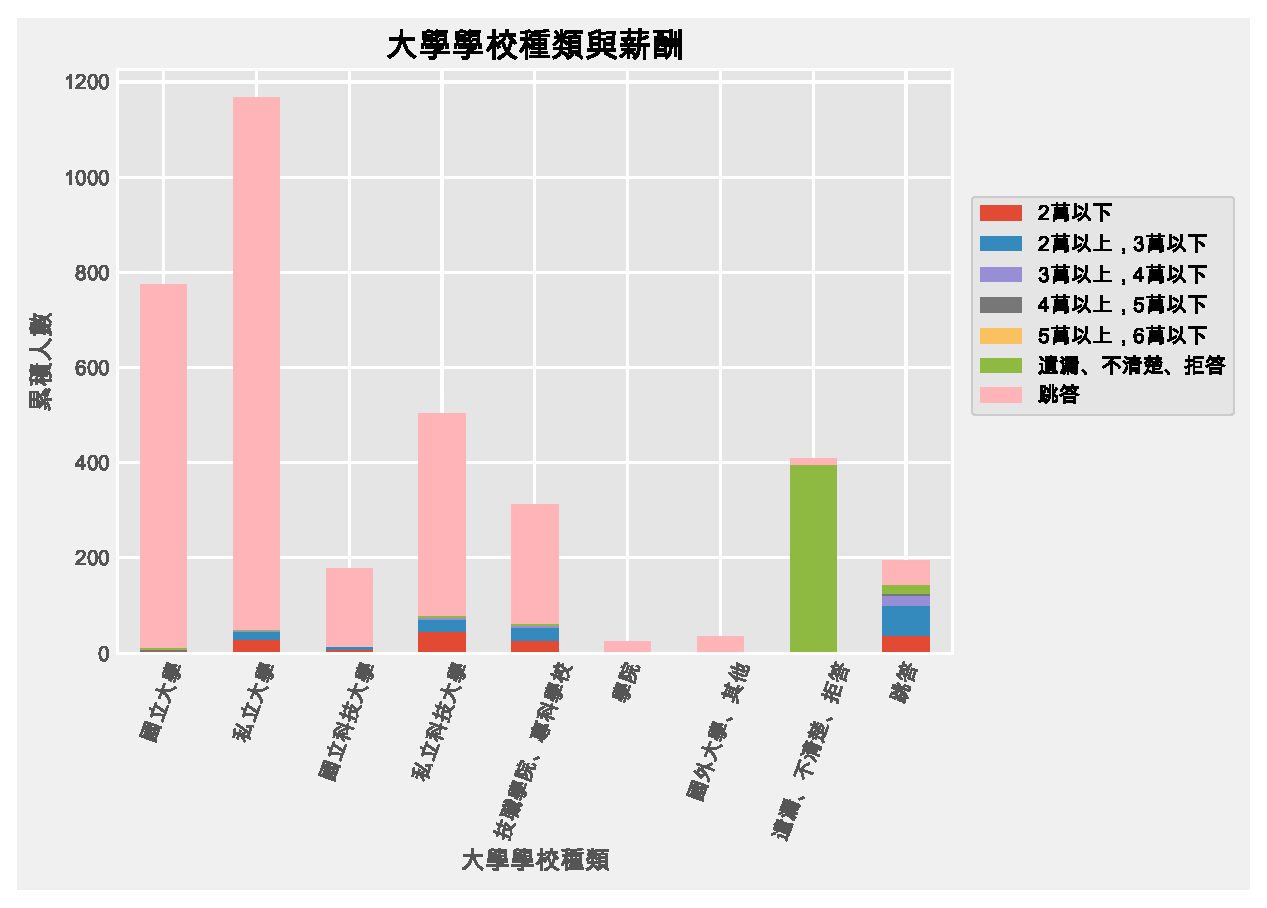
\includegraphics[width=\linewidth]{\imgdir/school_type_salary.eps}
        \caption{學校種類與薪酬}
        \label{pic:學校種類與薪酬}
\end{figure}

\begin{table}[ht]
\centering
\renewcommand{\arraystretch}{1.3} %%%把表格的高拉大
\extrarowheight=4pt
\begin{adjustbox}{width=\textwidth}
\begin{tabular}{l*{8}{c}}
\toprule
& \multicolumn{8}{c}{薪酬經過重新分組} \\
\cmidrule(lr){2-9}
大學學校種類 & 2萬以下 & 2萬以上& 3萬以上 & 4萬以上 & 5萬以上 & 遺漏、 & 跳答 & Total \\
		   &    &-3萬以下    & -4萬以下  &- 5萬以下    & -6萬以下   & 不清楚、拒答   &   &  \\
\midrule
國立大學 & 5 & 3 & 0 & 0 & 0 & 3 & 763 & 774 \\
私立大學 & 28 & 17 & 2 & 0 & 0 & 2 & 1,118 & 1,167 \\
國立科技大學 & 7 & 6 & 0 & 0 & 0 & 1 & 163 & 177 \\
私立科技大學 & 46 & 24 & 4 & 0 & 0 & 6 & 423 & 503 \\
技職學院、專科學校 & 27 & 27 & 4 & 0 & 1 & 3 & 250 & 312 \\
學院 & 0 & 1 & 0 & 0 & 0 & 0 & 23 & 24 \\
國外大學、其他 & 0 & 0 & 0 & 0 & 0 & 0 & 34 & 34 \\
遺漏、不清楚、拒答 & 1 & 1 & 0 & 0 & 0 & 395 & 11 & 408 \\
跳答 & 37 & 62 & 23 & 3 & 1 & 18 & 50 & 194 \\
Total & 151 & 141 & 33 & 3 & 2 & 428 & 2,835 & 3,593 \\
\bottomrule
\end{tabular}
\end{adjustbox}
\caption{薪酬經過重新分組的表格}
\end{table}








\end{document}
